\documentclass[conference]{IEEEtran}
\IEEEoverridecommandlockouts
% The preceding line is only needed to identify funding in the first footnote. If that is unneeded, please comment it out.
\usepackage{cite}
\usepackage{amsmath,amssymb,amsfonts}
\usepackage{algorithmic}
\usepackage{graphicx}
\usepackage{textcomp}
\usepackage{xcolor}
\def\BibTeX{{\rm B\kern-.05em{\sc i\kern-.025em b}\kern-.08em
    T\kern-.1667em\lower.7ex\hbox{E}\kern-.125emX}}
    
% my packages

\usepackage[ruled,vlined,linesnumbered]{algorithm2e}
\usepackage{tikz}
\usepackage{pgfplots}
\usepgfplotslibrary{groupplots}
\pgfplotsset{compat=1.17} 
\usepackage[caption=false]{subfig}


% \usepackage{tikz}
\usetikzlibrary{shapes.arrows,chains}
% \usepackage[ngerman]{babel}
\usepackage{babel}
\usetikzlibrary{decorations.pathreplacing,calligraphy,backgrounds}

\pagestyle{plain}


\title{gpupaper}
\author{kchiu }
\date{May 2021}

\begin{document}
\begin{figure}
    \centering
    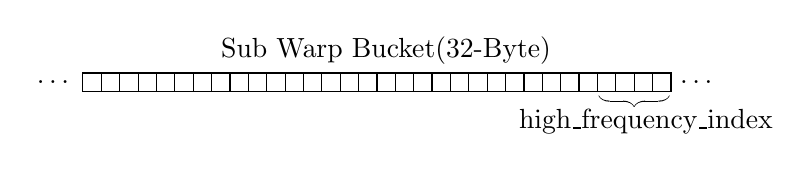
\begin{tikzpicture}[
          start chain=1 going right,start chain=2 going below,node distance=-0.15mm
        ]
        \node [on chain=2] at (2.7, 0) {Sub Warp Bucket(32-Byte)};
        \node [on chain=1] at (-1.5,-.4) {\ldots};  
        \foreach \x in {1,2,...,32} {
            \x, \node [draw,on chain=1] {};
            
        } 
        \node [name=r,on chain=1] {\ldots}; 
        \draw [name=b,white,decorate, decoration = {calligraphic brace, raise = 2pt, amplitude = 4pt,mirror}] (5.4,-0.5) --  (6.3,-0.5);
        \node at (6.0,-0.9) {high\_frequency\_index};
    \end{tikzpicture}
    \caption{Three simple graphs}
    \label{fig:graphs}
\end{figure}

\begin{figure}
     \centering
     \subfloat[a\label{1a}]
     {
           \resizebox{0.48\columnwidth}{!}{
           \begin{tikzpicture}%[scale=0.48]
            \label{fig:thread_perf_m_0.5}
            \begin{semilogxaxis}[
                title={Insert Performance for Different m},
                xlabel={Work Load},
                ylabel={Insert Performance (M operations/s)},
                legend pos=north east,
                xmajorgrids=true,
                ymajorgrids=true,
            ]
                \addplot table[x = WorkLoad, y = m1_insert] {data/qsketch/perf_m_0.5_r.dat};
                \addlegendentry{m == 1}
                \addplot table[x = WorkLoad, y = m2_insert] {data/qsketch/perf_m_0.5_r.dat};
                \addlegendentry{m == 2}
                \addplot table[x = WorkLoad, y = m3_insert] {data/qsketch/perf_m_0.5_r.dat};
                \addlegendentry{m == 3}
            \end{semilogxaxis}
        \end{tikzpicture}
            }
     }
     ~
     \hfill
     \subfloat[b\label{1b}]
     {
        \resizebox{0.48\columnwidth}{!}{
        \begin{tikzpicture}%[scale=0.48]
            \begin{semilogxaxis}[
                title={Search Performance for Different m},
                xlabel={Work Load},
                ylabel={Search Performance (M operations/s)},
                legend pos=north east,
                xmajorgrids=true,
                ymajorgrids=true,
            ]
                \addplot table[x = WorkLoad, y = m1_search] {data/qsketch/perf_m_0.5_r.dat};
                \addlegendentry{m == 1}
                \addplot table[x = WorkLoad, y = m2_search] {data/qsketch/perf_m_0.5_r.dat};
                \addlegendentry{m == 2}
                \addplot table[x = WorkLoad, y = m3_search] {data/qsketch/perf_m_0.5_r.dat};
                \addlegendentry{m == 3}
            \end{semilogxaxis}
        \end{tikzpicture}
        }
     }
        \caption{Three simple graphs}
        \label{fig:graphs2}
\end{figure}

Figure \ref{fig:graphs2} shows that
\end{document}
